% \begin{figure}
%     \centering
%     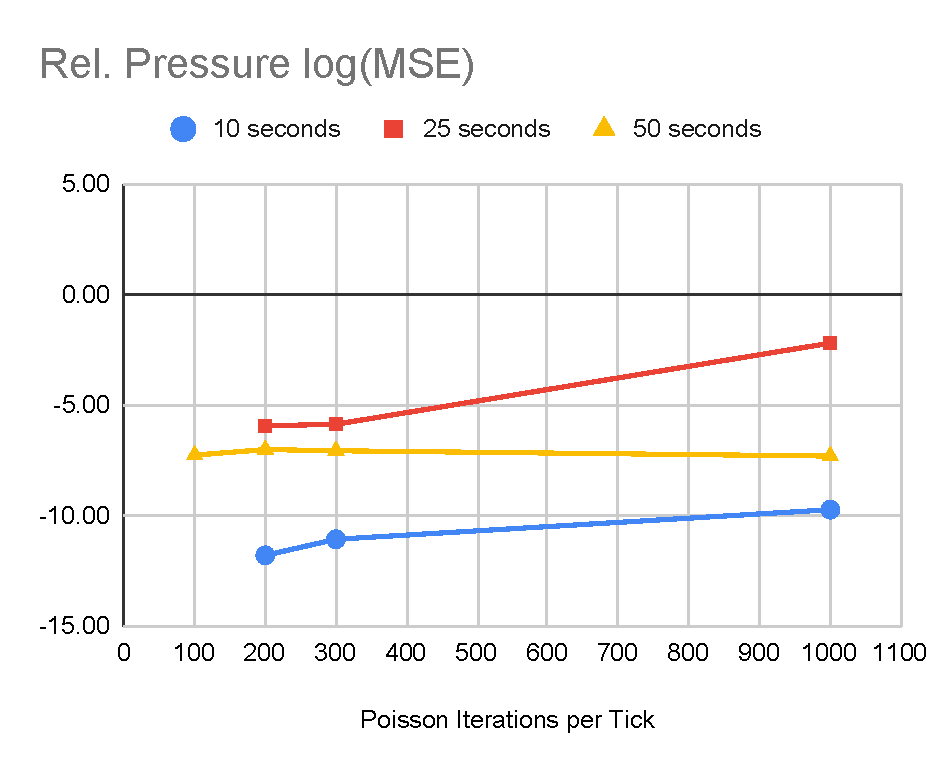
\includegraphics[width=0.5\linewidth]{Ch62Results/figures/temp_rel_pressure_mse.pdf}
%     \caption{MSE for Pressure when adjusted to use relative values}
%     \label{fig:results:mse_rel_pressure}
% \end{figure}

\begin{figure}
    \centering
    \begin{tikzpicture}
    \begin{axis}[
        title={Pressure (Relative) MSE},
        ylabel={MSE (log scale)},
        xlabel={Poisson Iterations per Tick},
        ymin=-15, ymax=5,
        xmin=0, xmax=1100,
        xtick={100,200,300,1000},
        ytick={5,0,-5,-10,-15},
        extra y ticks = {0},
        extra y tick labels = {},
        extra tick style = {
            grid=major,
            major grid style={line width=.5pt, draw=black}
        },
        yticklabels={$10^5$, $10^{0}$, $10^{-5}$, $10^{-10}$, $10^{-15}$},
        width=\linewidth,
        height=15em,
        legend pos = north east
    ]
    \addplot table [x=iters, y=pres-mean-10, col sep=space] {Ch62Results/figures/data/MSE.csv};
    % \addlegendentry{\SI{10}{\second}};
    \addplot table [x=iters, y=pres-mean-25, col sep=space] {Ch62Results/figures/data/MSE.csv};
    % \addlegendentry{\SI{25}{\second}};
    \addplot table [x=iters, y=pres-mean-50, col sep=space] {Ch62Results/figures/data/MSE.csv};
    % \addlegendentry{\SI{50}{\second}};
    \end{axis}
    \end{tikzpicture}
    \caption{MSE for Pressure when adjusted to use relative values}
    \label{fig:results:mse_rel_pressure}
\end{figure}


